%!TEX root = ../thesis.tex
\chapter{Applications \& Discussion}

This chapter presents a discussion of MapperGUI's software design and its consequences for musical mapping, as well as revisions made to the code since its initial release. The interface's features are explored in an attempt to evaluate the successes and failures of the design. Feedback from users was gathered throughout the project as well as through informal interviews after the software's release. This feedback is summarized and presented here. A modification to the code, motivated by feedback from users, is also described. MapperGUI is then compared to similar interfaces, analyzing especially new features that could be incorporated into our flexible framework. Finally, the system is evaluated overall with respect to the project's initial goals.


%%%%%%%%%%%%%%%%%%%%%%%%%%%%%%%%%%%%%%%%%%%%%%%%%%%%%%%%%%%%%%%%%%%%%%%%%%%%%%%%%%%%%%%%%%%%%%%%%%%%%%%%%%%%%%%%%%%%%%%%%%%%%%%%%%%%%%%%%%%%%%%%%%%%%%%%%%%%%%%%%%%%%%%%%%%%%%%%%%%%%%%%%%%%%%%%%%%%%%%%%%%%%%%%%%%%%%%%%%%%%%%%%%%%%%%%%%%%%%%%%%%%%%%%%%%%%%%%%%
\section{User Feedback} % (fold)
\label{sec:user_feedback}

The entire MapperGUI project began with user feedback for prior libmapper GUIs. Throughout the design process, functional versions of MapperGUI were provided to libmapper users at the IDMIL. Their feedback was crucial to the evolution of the software. After the first official release of MapperGUI, long-term users were informally interviewed. These users were questioned specifically about their particular applications of MapperGUI.

Even at this early stage of release, users have already incorporated MapperGUI into a wide variety of projects. This reflects our initial assumptions that a successful GUI must be flexible. Throughout development, MapperGUI was used as an experimental tool and aid in designing DMIs. The interface was used in concert with motion capture systems, vibrotactile feedback and even was loaded onto a Raspberry Pi\footnote{Raspberry Pi | An ARM GNU/Linux box for \$25. Take a byte! [Online] Available: \url{http://www.raspberrypi.org}. Accessed August 1, 2013}. During this process, users encountered problems, had ideas for extensions and used the GUI in ways we could not have anticipated.



%for response to vibrotactile feedback in a motion-capture study. It was also used in a motion capture setting for the design of an interactive audio installation. In the latter situation MapperGUI was required to handle many signals per single device, as each person in the room required 25 three-dimensional markers (75 signals total). A DMI designer has been using MapperGUI to test mappings for her input device with a single sound synthesizer, each containing about 30 signals.

%MapperGUI is being used as a development tool as well. A programmer is attempting to build a software bridge between libmapper and the Arduino\footnote{}. She uses MapperGUI to test the robustness and effectiveness of the software, and has even successfully loaded the GUI onto a raspberryPI\footnote{}

%\begin{table}
%\begin{center}
%\begin{tabular}{l p{5cm} p{5cm}}
	%\hline\hline
	%user&use case&concerns\\
	%\hline
	%Mailis&Intonespacio&saving and loading\\
	%Hakon&Experimenting with vibrotactile feedback and motion capture systems&Switching between various mappings\\
	%Clayton&An interactive space using motion capture&Reliability of network\\
	%Julie&libmapper code for firmata&Speed of function (she's using a rasperry Pi)\\
	%\hline
	%Andrew Stuart&teaches class with libmapper&\\
	%Gestes (Marlon)&Performance, etc.&Hide unconnected\\
%\end{tabular}
%\end{center}	
%\end{table}
%
%Hakon Knutzen, Mailis Rodrigues, Clayton Mamedes, Julie Ren\'e
		%%Mailis, Clayton, Hakon, Julie


	\subsection{General feedback} % (fold)
	\label{sub:general_feedback}

Most of our users had experience with libmapper and had attempted to compile and use the library from scratch. Many commented on how well MapperGUI lowered the barriers to entry for non-technical users. Users who had never used libmapper before pointed out how much time had been saved in their work flow, as opposed to using hard-coding mappings.

The best reviewed feature of MapperGUI was the automatic linear scaling control found in the top bar. Some users previously detected signal minima and maxima by hand, then directly calculated and applied linear scaling functions. With MapperGUI, the task is trivially easy: one must simply enter the desired destination range and set the connection to the \emph{Calibrate} mode. Most of the ``magic'' in this feature is the result of the libmapper API, but providing users access through an easy-to-use GUI is also important. One user expressed frustration because she was not aware this feature existed and instead continued to painstakingly condition her signals in Max/MSP. She was very impressed with how much time was saved by switching this workload to libmapper and MapperGUI.

Use of the other connection modes was rare. Users found the expression input box difficult and opaque. Directly calculating the appropriate mathematical expression was seen as too abstract. This is a sensible problem to have, as difficult text-based input is precisely the thing that MapperGUI is designed to avoid. One user suggested a two-dimensional graphical tool, showing the transposition from input to output would help with this task. 

Some users requested that signal values themselves be available in MapperGUI. This would create a lot of bandwidth clutter, as all devices would need to constantly send data to the GUI. It was suggested that the user could be able to query signal data by clicking or placing the mouse cursor over signal names.
	
	% subsection other_feedback (end)

	\subsection{Saving \& loading} % (fold)
	\label{sub:saving_and_loading}

Nearly all users made use of the saving and loading features in some way. For both experimental and design-based setups, returning to prior mappings is very useful as it avoids the tedium of performing the same tasks repeatedly.

We received criticism for the na\"ive loading system. One user found it counterintuitive that mappings would accumulate when loading multiple files, as he required rapid switching between the same few mappings for his experiment. Once these mappings were created, there was little that needed modification. For the experiment, it became tedious to erase a previous mapping before loading a new one. In a live-performance context the amount of delay inherent in this task would be unacceptable. 

Another user wished to switch between mappings in his work, but required some kind of intermediate space between the states. Each mapping represented a phase of a performance with a novel DMI. For this application, loading would ideally have the option of blending between two mappings such that the transition is not perceived as too sudden or harsh. To maintain this functionality, the actual saving and loading of patches was transferred to Max/MSP for his project, significantly reducing the utility of MapperGUI.

In a situation with many devices of the same class, loading a single mapping can be somewhat absurd. Because each connection will be loaded $m*n$ times (where $m$ is the number of similarly named input devices and $n$ is the number of relevant output devices), certain simple mappings can result in hundreds of unwanted connections upon loading. Perhaps some kind of staging area wherein the user can explicitly designate devices to use could solve this problem.

Another user asked for some kind of mapping preset that could be created and loaded whenever the program is opened. With this feature, if the same experiment is conducted repeatedly, the user would simply need to launch MapperGUI and begin to work.
	
	% subsection saving_&_loading (end)

	\subsection{Reliability \& responsiveness} % (fold)
	\label{sub:reliability_and_responsiveness}

Multiple users commented on the frustrating nature of interacting with MapperGUI when it became out of sync with the libmapper network. As one user stated, ``The program is not useful if you do not \emph{trust} the display.'' In this way small errors (devices not appearing, signals not accepting connections, delays in operations, etc.) become a very big issue for user satisfaction. Users reviewed the refresh button very favorably. If something seemed amiss with the GUI or the network and refreshing the display solved the problem, then trust in the display was restored.

Some problems were due to errors in the libmapper code and were out of the domain of MapperGUI. Others were created when MapperGUI code started to make assumptions about the libmapper network. For example, with the original drag-to-connect gesture, the drawn arrow persisted upon release of the mouse button. MapperGUI assumed that a connection would be made and kept the arrow to avoid delays. Occasionally, the signals were \emph{not} connected due to dropped messages or incompatibility. In these instances the faulty arrow, representing nothing, became very confusing. Due to negative feedback, the code was changed such that a drawn arrow disappears immediately after the drawing gesture. If the connection is successful, it is redrawn. This results in a slight flicker as the arrow is erased and re-drawn, but this was much more popular than potential erroneous arrows persisting in the display.

Some heavy operations, like scrolling and forming multiple connections, could create significant delays in MapperGUI. Users responded very negatively to such delays, as they were accustomed to computer programs responding much faster. Generally, multi-second delays were thought to be errors, thus reducing the user's trust in the application. We explore solutions to this problem in Section \ref{sec:testing_program_responsiveness}.
	
	% subsection reliability_and_responsiveness (end)

	\subsection{Effectiveness of alternate views} % (fold)
	\label{sub:effectiveness_of_alternate_views}

GridView and HiveView have only recently been included into the program. As a result, most of our users were much more familiar with ListView. Users reported that while the alternate views were interesting, ListView was the most straightforward for creating mappings. It was reported that GridView could be interesting once most of the mapping was completed, as one could notice patterns that were not apparent in ListView. The limited functionality of HiveView meant that, to most users, it was simply a visualization tool. It was also extremely common among our test users for use cases to include very few devices with many connections, meaning that the ``whole-network'' view in HiveView was not advantageous.
	
	% subsection effectiveness_of_alternate_views (end)
	
% section user_feedback (end)

%%%%%%%%%%%%%%%%%%%%%%%%%%%%%%%%%%%%%%%%%%%%%%%%%%%%%%%%%%%%%%%%%%%%%%%%%%%%%%%%%%%%%%%%%%%%%%%%%%%%%%%%%%%%%%%%%%%%%%%%%%%%%%%%%%%%%%%%%%%%%%%%%%%%%%%%%%%%%%%%%%%%%%%%%%%%%%%%%%%%%%%%%%%%%%%%%%%%%%%%%%%%%%%%%%%%%%%%%%%%%%%%%%%%%%%%%%%%%%%%%%%%%%%%%%%%%%%%%%
\section{Improving Program Responsiveness} % (fold)
\label{sec:testing_program_responsiveness}

The extension of interface features discussed in Section \ref{sec:extension_of_control_and_visual_elements} leads to some control possibilities that could be difficult for MapperGUI to handle. The addition of shortcut keys and multiple selection allows users to create and delete hundreds of connections with a single key press. Na\"{i}ve saving and loading produces situations where dense mappings will accidentally be applied to several instruments at once.

Though the \url{view.update_display} technique works extremely well for code modularity, it generates awkward situations when dealing with massive network operations. Since the system updates the entire display with each change to the network, deleting 100 links (if the user is clearing a large network) results in 100 independent \url{delete_link} messages arriving at the monitor. For each one of these messages, the display will fully re-draw itself. In the case of ListView, all arrows will be cleared and redrawn with one fewer present, as if the links are being deleted one by one. In total, 4950 arrow drawing operations\footnote{$99 + 98 + 97 + ... + 2 + 1 = \frac{99*100}{2}$. Note that $\frac{n*(n+1)}{2}$ arrows will be drawn for any $n$ number of connections or links.} will occur when deleting 100 objects, resulting in a significant delay. 

As reported by users in Section \ref{sub:reliability_and_responsiveness}, any GUI operation that takes more than a few moments without some kind of visual feedback (like a ``loading'' bar) leads to frustration and mistrust of the program. If the GUI is going to support these kinds of massive network manipulations, there needs to exist some way to keep them under control.

	\subsection{Rate limiting functions} % (fold)
	\label{sub:rate_limiting_certain_functions}

In order to prevent thousands of unnecessary display re-draws, a ``waiting'' period was added to certain critical functions \shortcite{os_concepts}. These functions no longer execute immediately once called. Instead, a delay timer starts. If the function is called again during this delay, the delay timer simply restarts. The function is only executed once the delay timer finishes. This way, if a function is called 100 times simultaneously, it will only execute once after a short delay. Figure \ref{fig:waiting_period} shows the effect of the waiting period.

\begin{figure}
	\centering
		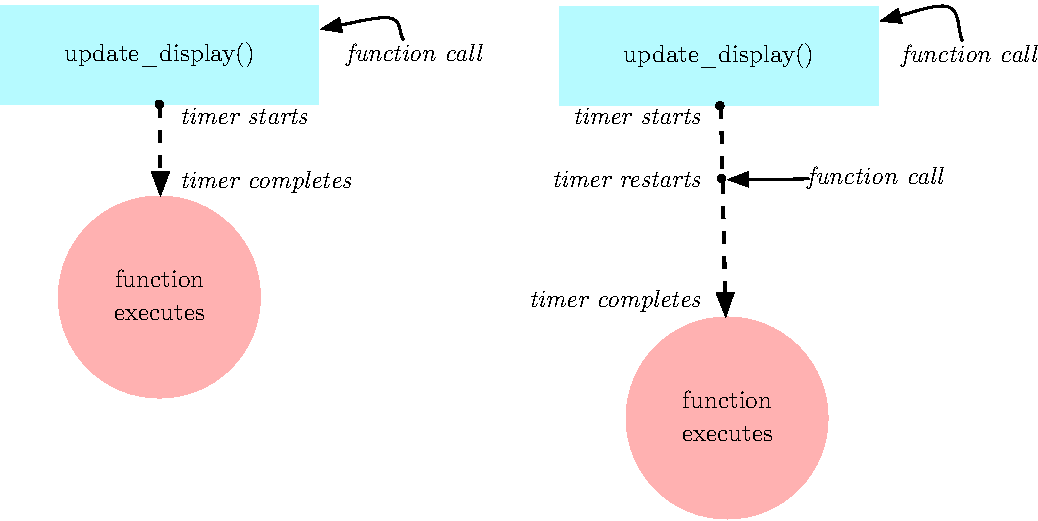
\includegraphics[width=1\textwidth]{figures/waiting_period}
		\caption{Illustration of a delayed function.}
		\label{fig:waiting_period}
\end{figure}

%Two functions are limited in the GUI: \url{view.update_display} for all views and \url{update_arrows} for ListView. \url{update_display} is common to all views, and the massive network changes described above can result in many processor intesive functions to run needlessly. With the \url{update_arrows} function, operations that do not result in changes to the network (scrolling, changing tabs) require constant re-drawing.

Exactly how much time this delay should be set to is not obvious. If the delay is too short, it is possible for massive network operations to still cause multiple redundant display updates. A delay that is too long means that users may perceive the delays for simple actions, like creating a single arrow. Another consequence of a long delay is that a process which calls the delayed function at a regular interval could continuously restart the tomer. In this case, the function will \emph{never} execute, a situation known as ``starvation.''

After some informal tests of delays between 17 and 1000 milliseconds, a delay of 33 milliseconds was selected for both functions. Substantial improvement in execution speed was observed for even very short delays, as often hundreds of function calls would reach the \url{view.update_display} pracitcally simultaneously. With delays closer to one second, we saw little improvement in response to massive network operations and the delay itself became noticeable. 33 milliseconds is in the range where nearly every operation results in a single function execution and is imperceptible to a human user. The number 33 itself was selected because it is the length of two screen refreshes on a 60 Hz display (a measure recommended by \shortciteANP{os_concepts}).
	
	% subsection rate_limiting_certain_functions (end)

% section testing_program_responsiveness (end)

%%%%%%%%%%%%%%%%%%%%%%%%%%%%%%%%%%%%%%%%%%%%%%%%%%%%%%%%%%%%%%%%%%%%%%%%%%%%%%%%%%%%%%%%%%%%%%%%%%%%%%%%%%%%%%%%%%%%%%%%%%%%%%%%%%%%%%%%%%%%%%%%%%%%%%%%%%%%%%%%%%%%%%%%%%%%%%%%%%%%%%%%%%%%%%%%%%%%%%%%%%%%%%%%%%%%%%%%%%%%%%%%%%%%%%%%%%%%%%%%%%%%%%%%%%%%%%%%%%
\section{Comparison to Similar Interfaces} % (fold)
\label{sec:comparison_to_similar_interfaces}

Other systems exist to help non-programmers map control inputs to sound synthesis parameters. This section compares this research to these systems, some of which are paid software.

\begin{figure}[h]
	\centering
		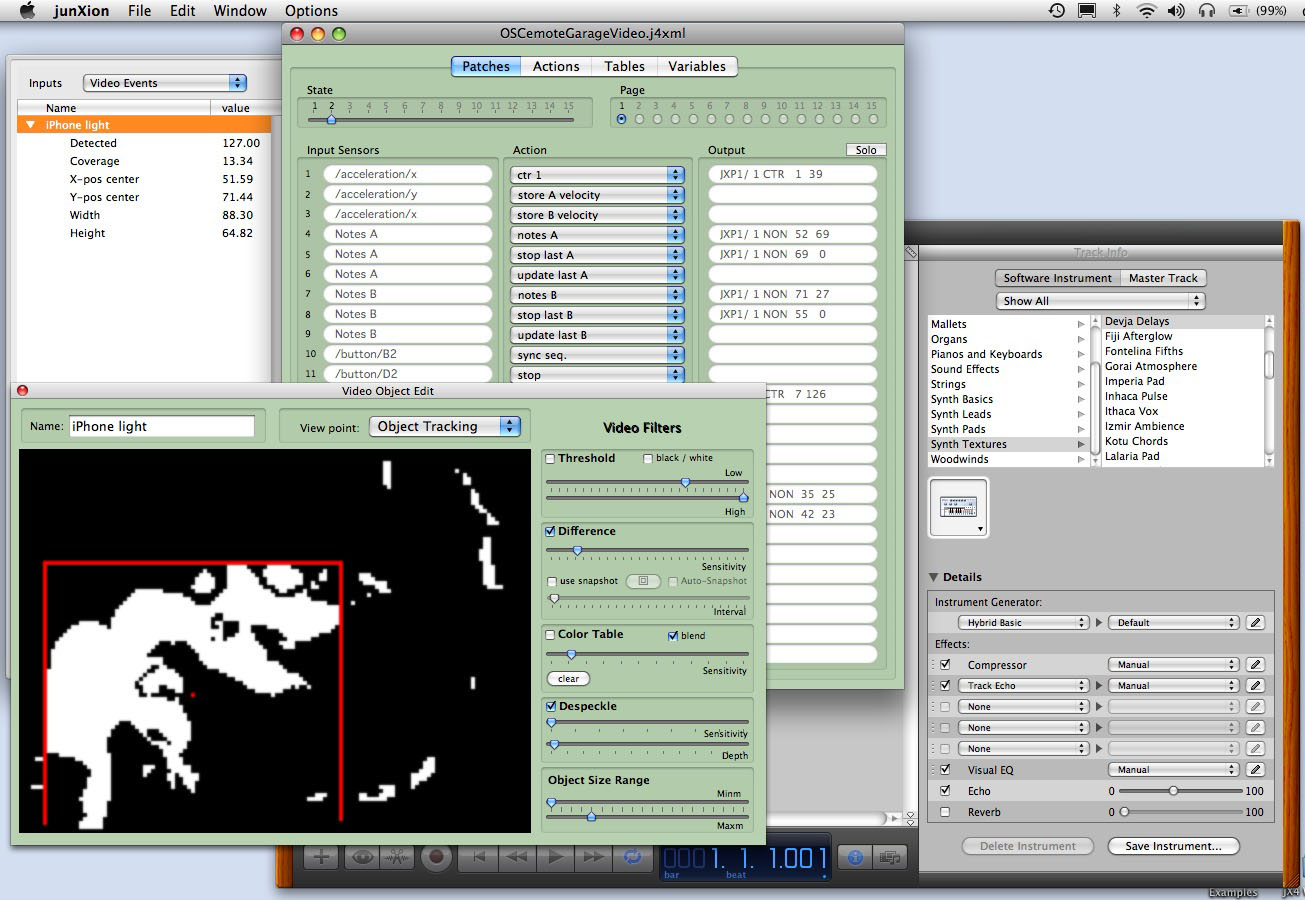
\includegraphics[width=\textwidth]{figures/junXion_v4}
		\caption{STEIM's JunXion software}
		\label{fig:junxion}
\end{figure}

The Studio for Electro-Instrumental Music (STEIM) distributes JunXion \cite{junxion}, a software application for controlling MIDI and OSC-based systems. JunXion automatically detects input devices like computer mice and USB video-game controllers. The user is able to drag child signals from these controllers onto one of 25 possible inputs.  From there users can switch to the ``actions'' tab, where destinations and connection properties can be customized. The program stores connection properties in groups that populate drop-down menus in the central column. JunXion features a very interesting ``state'' system similar to MapperGUI's saving and loading. Once a successful mapping is created, users can change the state, which starts a new mapping. With multiple mappings, users can quickly switch between states. JunXion also has a very interesting graphical signal conditioning editor. The program presents a two dimensional field and the user can draw, generate curves and set bounds. Incorporating such a feature into MapperGUI would assist users who are unimpressed by textual expression input.

\begin{figure}[h]
	\centering
		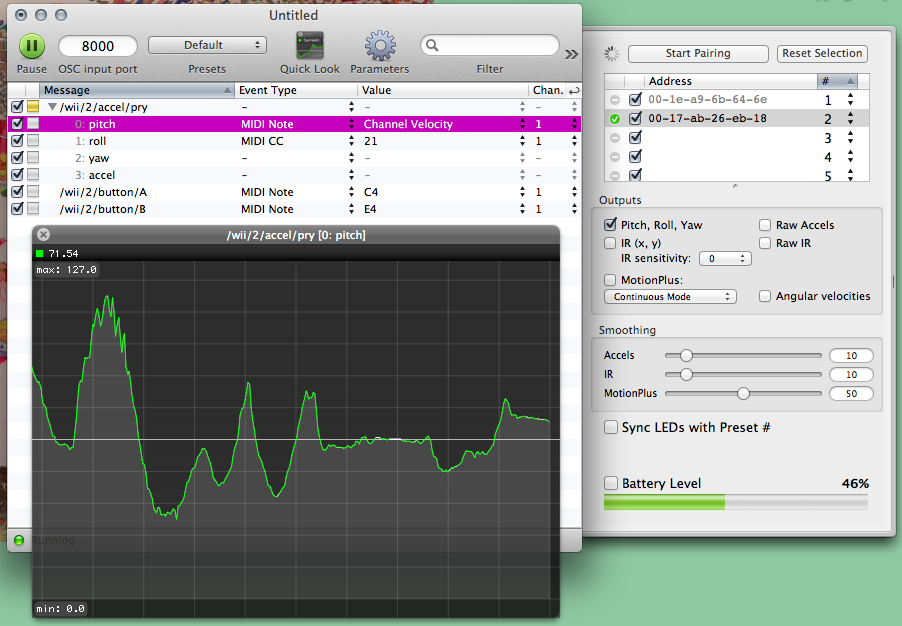
\includegraphics[width=\textwidth]{figures/osculator}
		\caption{The OSCulator interface}
		\label{fig:osculator}
\end{figure}

The OSCulator system \cite{osculator} is very similar to JunXion. Compatible controllers appear automatically and can be mapped to MIDI or OSC signals. OSCulator also relies on a drop-down menu based interface for selecting where and how the output will be routed. As in JunXion, the idea of a ``connection'' is not emphasized. Instead, a MIDI or OSC message is simply sent on a specific channel (the receiving end must be notified on which channel to receive messages). As can be seen in Figure \ref{fig:osculator}, OSCulator displays a real-time oscilloscope-like visualization for selected signals. A similar feature would improve MapperGUI's visual feedback, though it would require actual signal data from libmapper.

The Eaganmatrix \cite{eaganmatrix} partly inspired GridView in MapperGUI. The signals of a single control and synthesis device are displayed on the x and y axes of a grid display. Connections between the two are made by clicking on the intersections. The Patchage interface \cite{patchage} contains an interaction very similar to ListView: objects containing lists of signals can be connected by dragging gestures. Max/MSP and Integra Live \cite{integra} also feature this interaction, but neither are necessarily for creating mappings. 

	% subsection other_similar_interfaces (end)

% section comparison_to_similar_interfaces (end)

%%%%%%%%%%%%%%%%%%%%%%%%%%%%%%%%%%%%%%%%%%%%%%%%%%%%%%%%%%%%%%%%%%%%%%%%%%%%%%%%%%%%%%%%%%%%%%%%%%%%%%%%%%%%%%%%%%%%%%%%%%%%%%%%%%%%%%%%%%%%%%%%%%%%%%%%%%%%%%%%%%%%%%%%%%%%%%%%%%%%%%%%%%%%%%%%%%%%%%%%%%%%%%%%%%%%%%%%%%%%%%%%%%%%%%%%%%%%%%%%%%%%%%%%%%%%%%%%%%
\section{Summary \& Evaluation of Goals} % (fold)
\label{sec:evaluation_of_goals}

A set of goals for the software was established at the beginning of this document. These were to create an interface for libmapper that was easy to use and to make this interface modular and multi-platform. Creating a system that was flexible and intuitive was of primary concern. We also intended to unite features of the three prior GUIs, both to capitalize on work already completed and create a single, standard graphical interface for libmapper. 

Our GUI currently exists in a distributable form, allowing Macintosh users to download and use the software easily. Unfortunately, standalone applications for non-Macintosh platforms are not yet available. Most features from prior interfaces were integrated into a cross-compatible web-based system. A modular codebase was created for the application, greatly improving the processes of maintaining and extending this GUI versus prior interfaces. Two new view modes were integrated into the display, though it is too early to conclude as to whether they significantly contribute to the flexibility of the system.

The software was provided to users, and thus tested in a variety of contexts. MapperGUI was able to handle most use cases in its present state. All shortcomings were recorded and those that have not yet been addressed are listed along with possible solutions in Section \ref{sec:future_work}. Though it has not yet been the case, MapperGUI will likely be used to handle mappings in live performance contexts in the future. This will give us a new perspective on how the software performs in a situation where instant reactivity is a necessity and errors can be disastrous. 
	
% section evaluation_of_goals (end)




